\documentclass{article}
\usepackage[paperwidth=18cm,paperheight=27cm,margin=5mm]{geometry}
\usepackage{graphicx}
\usepackage{tikz}
\usepackage[hidelinks]{hyperref}
\setlength{\parindent}{0pt}
\pagestyle{empty}

% The source image is 1024 x 1536 px and is displayed at 17 cm wide.
% Each hotspot is an invisible clickable rectangle over the matching block.
\newcommand{\hotspot}[5]{%
  \node[anchor=south west,inner sep=0pt,outer sep=0pt] at (#2,#3) {%
    \hyperlink{#1}{\phantom{\rule{#4cm}{#5cm}}}%
  };%
}

\begin{document}
\hypertarget{diagram-top}{}
\noindent
\begin{tikzpicture}[x=0.0166015625cm,y=0.0166015625cm]
  \node[anchor=south west,inner sep=0pt] at (0,0)
    {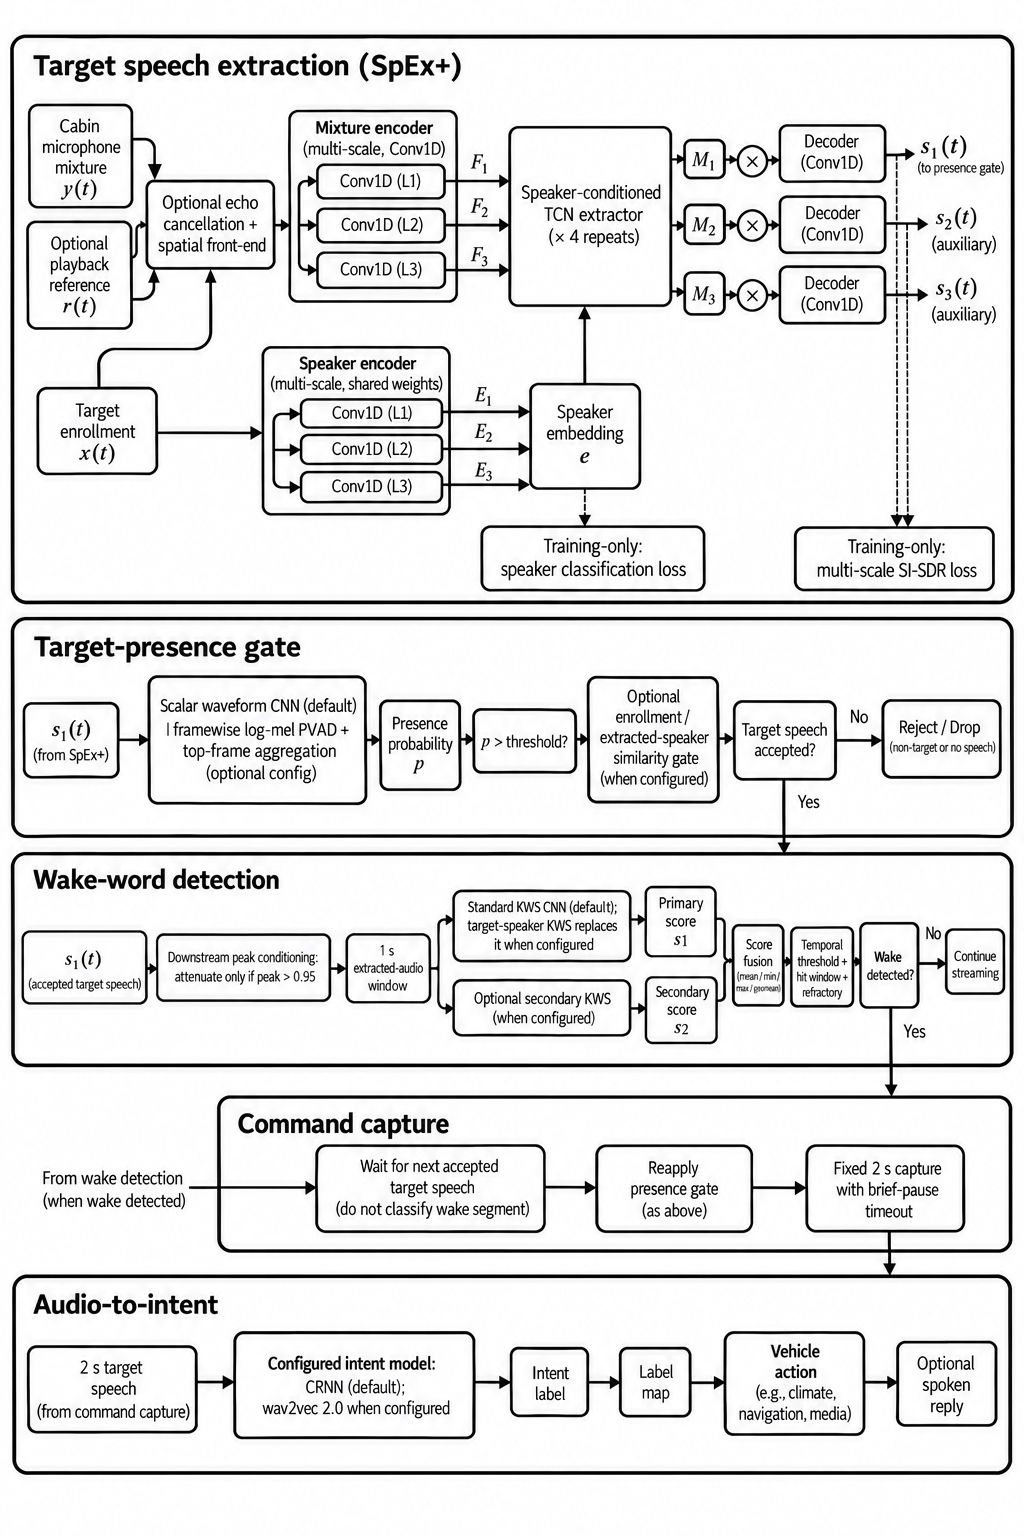
\includegraphics[width=17cm]{fig1_system_runtime.png}};

  % Hotspots use bottom-left image coordinates in pixels.
  \hotspot{speaker-extractor}{508}{1229}{2.72}{3.00}
  \hotspot{presence-gate}{147}{731}{3.65}{2.14}
  \hotspot{primary-kws}{452}{573}{3.04}{1.22}
  \hotspot{secondary-kws}{452}{498}{3.04}{0.98}
  \hotspot{command-capture}{315}{303}{3.82}{1.50}
  \hotspot{intent-classifier}{234}{98}{4.00}{1.76}
  \hotspot{training-losses}{480}{944}{8.55}{1.06}
\end{tikzpicture}

\clearpage
\pagestyle{plain}
\section*{Using the interactive diagram}
Hover over a linked block to reveal the PDF link cursor; click it to jump to its explanation.
Use the return link at the end of each explanation to go back to the diagram.

\hypertarget{speaker-extractor}{\section*{Speaker extractor}}
The SpEx+ stage encodes the cabin mixture and the target enrollment at three temporal scales. The enrollment representation conditions a repeated temporal-convolution extractor, which estimates one mask per scale. Applying those masks to the mixture features and decoding them produces \(s_1\), \(s_2\), and \(s_3\). Runtime inference forwards \(s_1\); the other outputs support the multi-scale training objective.

\hypertarget{presence-gate}{\section*{Target-presence gate}}
The configured presence head estimates whether target speech is present in the extracted waveform. The scalar waveform CNN is the default; a framewise log-mel PVAD head with top-frame aggregation is available as a configured alternative. An optional speaker-similarity gate can additionally compare the enrolled and extracted speaker representations. A rejected segment is dropped before wake-word processing.

\hypertarget{primary-kws}{\section*{Primary wake-word detector}}
The standard KWS CNN is the default detector. When the enrollment-conditioned target-speaker KWS model is configured, it replaces the standard primary detector. The primary score is evaluated over the extracted audio window.

\hypertarget{secondary-kws}{\section*{Secondary KWS and temporal decision}}
An optional secondary KWS model can contribute a second score. The pipeline combines primary and secondary scores using the configured fusion rule, then applies the wake threshold, temporal hit window, and refractory period. Without a wake decision, the stream continues.

\hypertarget{command-capture}{\section*{Post-wake command capture}}
A wake event arms a separate command-capture state. The wake-word segment itself is not sent to intent classification. The system waits for the next accepted target-speech segment, rechecks presence, allows a brief pause, and resets capture after the configured timeout.

\hypertarget{intent-classifier}{\section*{Audio-to-intent classifier}}
The next accepted command segment is prepared as a fixed two-second input. The CRNN is the default classifier; a wav2vec 2.0 encoder and classifier head can be selected by configuration. The predicted intent class is mapped to a vehicle action and may include a spoken reply.

\hypertarget{training-losses}{\section*{Training-only paths}}
The dotted connections in the diagram identify training supervision. Multi-scale SI-SDR loss supervises the extracted outputs, while speaker-classification loss supervises the speaker representation. These losses are not part of runtime inference.

\vfill
\hyperlink{diagram-top}{Return to the diagram}
\end{document}
